\documentclass[unicode]{beamer}
\usetheme{Madrid}
\usecolortheme{seahorse}     %цветовая схема
\useinnertheme{circles}   %внутренняя тема
\usefonttheme{serif}    %шрифты

\usepackage[utf8]{inputenc}
\usepackage[T2A]{fontenc}
\usepackage[russian]{babel}
\usepackage[listings,theorems]{tcolorbox}
\usepackage{caption}
\usepackage[labelsep=period]{caption}
\setbeamertemplate{caption}[numbered]
\graphicspath{{/Users/arsenytokarev/Desktop/LaTeX/Competing species /Pictures/}}

\definecolor{shBlue}{HTML}{d6d6f0}
\definecolor{lightGray}{HTML}{F5F5F5}
\definecolor{spGreen}{HTML}{93DDC2}
\definecolor{spBlue}{HTML}{007AFF}
\definecolor{mainBackground}{HTML}{F9FEFC}

\makeatletter
\newcommand*{\rom}[1]{\expandafter\@slowromancap\romannumeral #1@}
\makeatother


\setbeamercolor{block title}{bg=shBlue!70,fg=black}
\setbeamercolor{block body}{bg=lightGray!50,fg=black}
% \setbeamercolor{frametitle}{fg=selected,bg=spGreen}
% \setbeamercolor{background canvas}{bg=mainBackground}
\setbeamertemplate{blocks}[rounded][shadow=false]

\title[Курсовая работа]{Модель двух конкурирующих видов}
\author[Токарев~А.И.]{Токарев~А.И.}
\institute[]{МГТУ им. Н.Э. Баумана}
\date{\today}

\begin{document}

    \begin{frame}
        \titlepage
    \end{frame}

    \begin{frame}
        \frametitle{Содержание}
        \tableofcontents
    \end{frame}

    \section{Постановка задачи}
    \begin{frame}
        \frametitle{Постановка задачи}
        \begin{block}{Гипотезы}
            \fontsize{10.4pt}{12pt}\selectfont
            \begin{enumerate}
                \item Пища имеется в неограниченном количестве или ее поступление регулируется.
                \item В единицу времени погибает одинаковое количество особей одного вида.
                \item Прирост численности вида пропорционален его текущей численности.
            \end{enumerate}
        \end{block}

        \begin{block}{Модель В. Вольтерра о конкуренции двух видов}
            \fontsize{10pt}{12pt}\selectfont
            \begin{equation}
                \label{volterra}
                \begin{cases}
                    \dfrac{dx_1}{dt} = a_1 x_1 - b_{12} x_1 x_2 - c_1 {x_1}\!^2,
                    \\[1em]
                    \dfrac{dx_2}{dt} = a_2 x_2 - b_{21} x_2 x_1 - c_2 {x_2}\!^2 ,
                \end{cases}
            \end{equation}
            \noindent где $a_i$ --- скорость роста популяции; $b_{ij}$ --- межвидовая борьба; $c_i$ --- внутривидовая борьба.
        \end{block}
    \end{frame}

    \section{Стационарные состояния}

    \begin{frame}
        \frametitle{Стационарные состояния}

        Приравниваем каждое из уравнений системы \eqref{volterra} к нулю:
        \begin{equation}
            \label{nullclines}
            \begin{cases}
                a_1 x_1 - b_{12} x_1 x_2 - c_1 {x_1}\!^2 = x_1 (a_1 - b_{12} x_2 - c_1 x_1) = 0,
                \\[0.3em]
                a_2 x_2 - b_{21} x_2 x_1 - c_2 {x_2}\!^2 = x_2 (a_2 - b_{21} x_1 - c_2 x_2) = 0
            \end{cases}
        \end{equation}

        Из системы \eqref{nullclines} получаем уравнения четырех прямых-сепаратрис:
        \begin{block}{}
            \[
                x_1 = 0,\quad x_2 = \dfrac{a_1 - c_1 x_1}{b_{12}}
            \]
        \end{block}

        \begin{block}{}
            \[
                x_2 = 0,\quad x_2 = \dfrac{a_2 - b_{21} x_1}{c_2}
            \]
        \end{block}
    \end{frame}

    \begin{frame}
        Попарные пересечения прямых, полученных из системы \eqref{nullclines}, дают четыре стационарные точки.
        \begin{block}{Cтационарные точки}
            \begin{enumerate}
                \setlength\itemsep{0.6em}
                \item[{\rom 1}] $ x_1 = 0,\ x_2 = 0 $ --- вымирание обоих видов.
                \item[{\rom 2}] $ x_1 = \dfrac{a_1}{c_1},\ x_2 = 0 $ --- противоположная ситуация, то есть достижение первым видом численности $ \dfrac{a_1}{c_1} $ и вымирание второго вида.
                \item[{\rom 3}] $ x_1 = 0,\ x_2 = \dfrac{a_2}{c_2} $ --- вымирание первого вида, достижение вторым видом конечной численности $ \dfrac{a_2}{c_2} $.
                \item[{\rom 4}] $ x_1 = \dfrac{a_1 c_2 - a_2 b_{12}}{c_1 c_2 - b_{12} b_{21}},\ x_2 = \dfrac{a_2 c_1 - a_1 b_{21}}{c_1 c_2 - b_{12} b_{21}}$ --- выживание обоих \\[0.5em] видов.
            \end{enumerate} 
        \end{block}
    \end{frame}

    \begin{frame}
        Система \eqref{volterra} является нелинейной. Линеаризуем ее в окрестности особых точек, чтобы определить их тип.
        \\[1.5em]
        $
            \mathbb{J} = 
            \begin{pmatrix}
                \dfrac{\partial{\dot x_1}}{\partial x_1}
                &
                \dfrac{\partial{\dot x_1}}{\partial x_2}
                \\[5mm]
                \dfrac{\partial{\dot x_2}}{\partial x_1}
                &
                \dfrac{\partial{\dot x_2}}{\partial x_2}
            \end{pmatrix}
        =
            \begin{pmatrix}
                a_1 - b_{12} x_2 - 2 c_1 x_1 & -b_{12} x_1
                \\
                -b_{21} x_2 & a_2 - b_{21} x_1 - 2c_2 x_2
            \end{pmatrix}\!.
        $
        \\[1.5em]
        $
            \mathbb{J}_{\rom 1} = 
                    \begin{pmatrix}
                        a_1 & 0
                        \\
                        0   & a_2
                    \end{pmatrix} \quad \Rightarrow \quad \lambda_1 = a_1,\  \lambda_2 = a_2.
        $
        \\[1.5em]
        $
            \mathbb{J}_{\rom 2} = 
                \begin{pmatrix}
                    -a_1 & -\dfrac{a_1 b_{12}}{c_1}
                    \\[4mm]
                    0   & \dfrac{a_2 c_1 - a_1 b_{21}}{c_1}
                \end{pmatrix} \quad \Rightarrow \quad \lambda_1 = -a_1,\  \lambda_2 = \dfrac{a_2 c_1 - a_1 b_{21}}{c_1}.
        $
    \end{frame}

    \begin{frame}
        $
            \mathbb{J}_{\rom 3} = 
            \begin{pmatrix}
                \dfrac{a_1 c_2 - b_{12} a_2}{c_2} & 0
                \\[4mm]
                -\dfrac{a_2 b_{21}}{c_2}          & -a_2
            \end{pmatrix} \quad \Rightarrow \quad \lambda_1 =  \dfrac{a_1 c_2 - b_{12} a_2}{c_2},\  \lambda_2 = -a_2.
        $
        \\[1.5em]
        $
        \mathbb{J}_{\rom 4} = 
            \begin{pmatrix}
                \dfrac{c_1 (a_1 c_2 - a_2 b_{12})}{b_{12} b_{21} - c_1 c_2} & \dfrac{b_{12} (a_1 c_2 - a_2 b_{12})}{b_{12} b_{21} - c_1 c_2}
                \\[4mm]
                \dfrac{b_{21} (a_2 c_1 - a_1 b_{21})}{b_{12} b_{21} - c_1 c_2}   & \dfrac{c_2 (a_2 c_1 - a_1 b_{21})}{b_{12} b_{21} - c_1 c_2}
            \end{pmatrix}\!.
        $
        \\[1.5em]
        Все стационарные точки являются простыми, поэтому их тип определяется собственными числами матриц $  \mathbb{J}_{{\rom 1}-{\rom 4}} $.
    \end{frame}

    \section{Сосуществование двух видов}
    \begin{frame}
        \frametitle{Сосуществование двух видов}
        Выживание обоих видов означает наличие неподвижной точки, обе координаты которой положительны, а также при условии, что:
        \[
            \begin{cases}
                a_1 c_2 > a_2 b_{12},
                \\
                a_2 c_1 > a_1 b_{21},
                \\
                c_1 c_2 > b_{12} b_{21}
            \end{cases}
        \]
        \begin{figure}
            \centering
            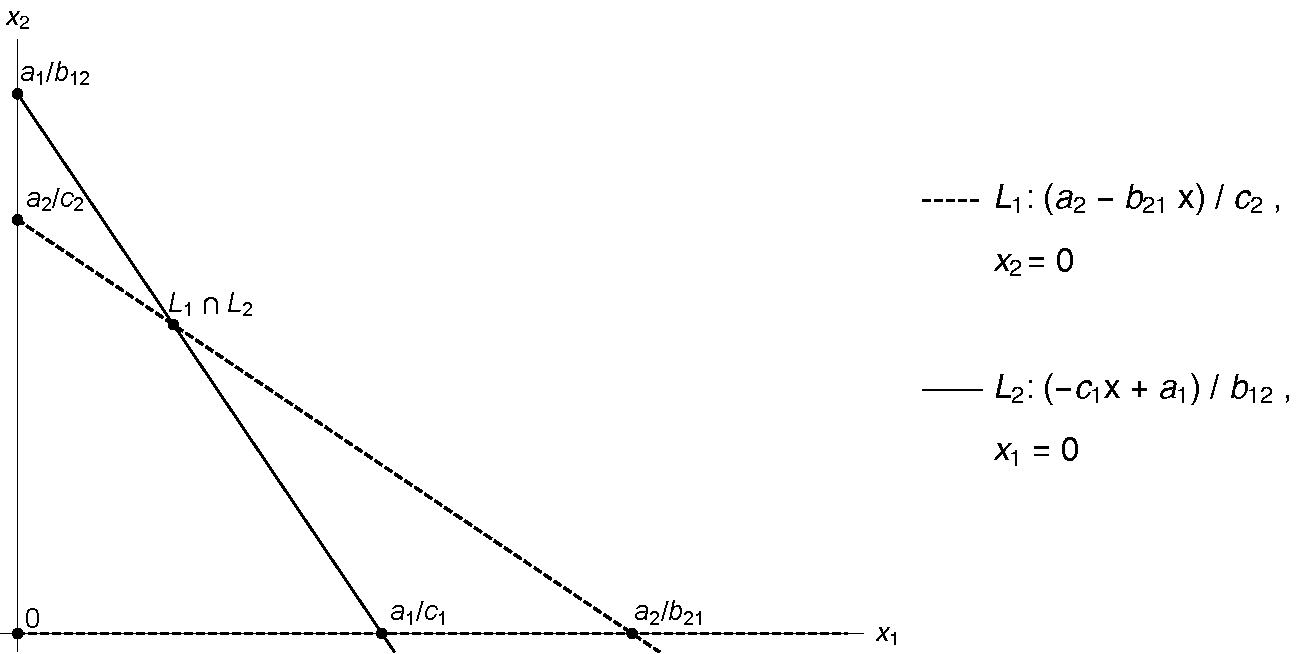
\includegraphics[width=0.6\textwidth]{sep_1.pdf}
            \caption{Расположение прямых при указанных коэффициентах}
        \end{figure}
    \end{frame}

    \begin{frame}
        \begin{enumerate}
            \setlength\itemsep{0.5em}
            \item[{\rom 1}] $ \lambda_1 = a_1 > 0,\ \lambda_2 = a_2 > 0 \Rightarrow $ точка $ {\rom 1} $ --- неустойчивый узел.
            \item[{\rom 2}] $ \lambda_1 = -a_1 < 0,\ \lambda_2 = \dfrac{a_2 c_1 - a_1 b_{21}}{c_1} > 0 \Rightarrow $ точка $ {\rom 2} $ --- седло.
            \item[{\rom 3}]  $ \lambda_1 = \dfrac{a_1 c_2 - b_{12} a_2}{c_2} > 0,\ \lambda_2 = -a_2 < 0 \Rightarrow $ точка $ {\rom 3} $ --- седло.
            \item[{\rom 4}]  $ \lambda_{1,2} < 0 \Rightarrow $  точка $ {\rom 4} $ --- устойчивый узел.
        \end{enumerate}

        \begin{figure}
            \centering
            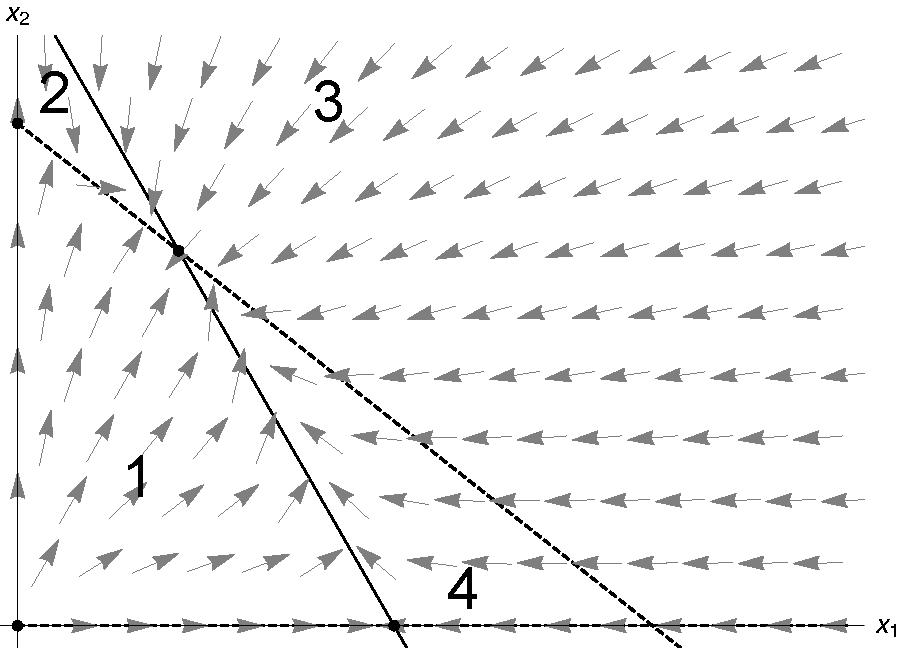
\includegraphics[width=0.5\textwidth]{areas_1.pdf}
            \caption{Поле направлений}
        \end{figure}
    \end{frame}

    \begin{frame}
        Построим окончательный фазовый портрет:
        \begin{figure}[h]
            \centering
            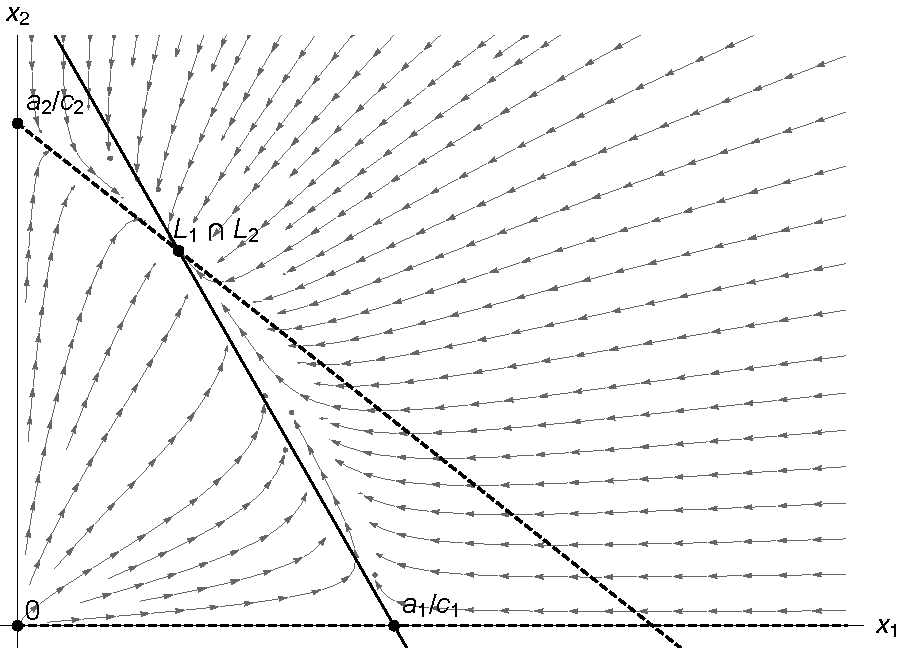
\includegraphics[width=0.6\textwidth]{phase_1.pdf}
            \caption{Сосуществование двух видов}
            \label{fig:phase_1}
        \end{figure}

        Из полученной картины можно сделать вывод, что сосуществование двух видов  гарантировано, потому что все траектории стремятся к 4-ой точке.
    \end{frame}

    \section{Выживание одного из видов в зависимости от начальных условий}
    \begin{frame}
        \frametitle{Выживание одного из видов}
        Также необходимо наличие особой точки, обе координаты которой положительны, но уже при других условиях:
        \[
            \begin{cases}
                a_1 c_2 < a_2 b_{12},
                \\
                a_2 c_1 < a_1 b_{21},
                \\
                c_1 c_2 < b_{12} b_{21}
            \end{cases}
        \]

        \begin{figure}
            \centering
            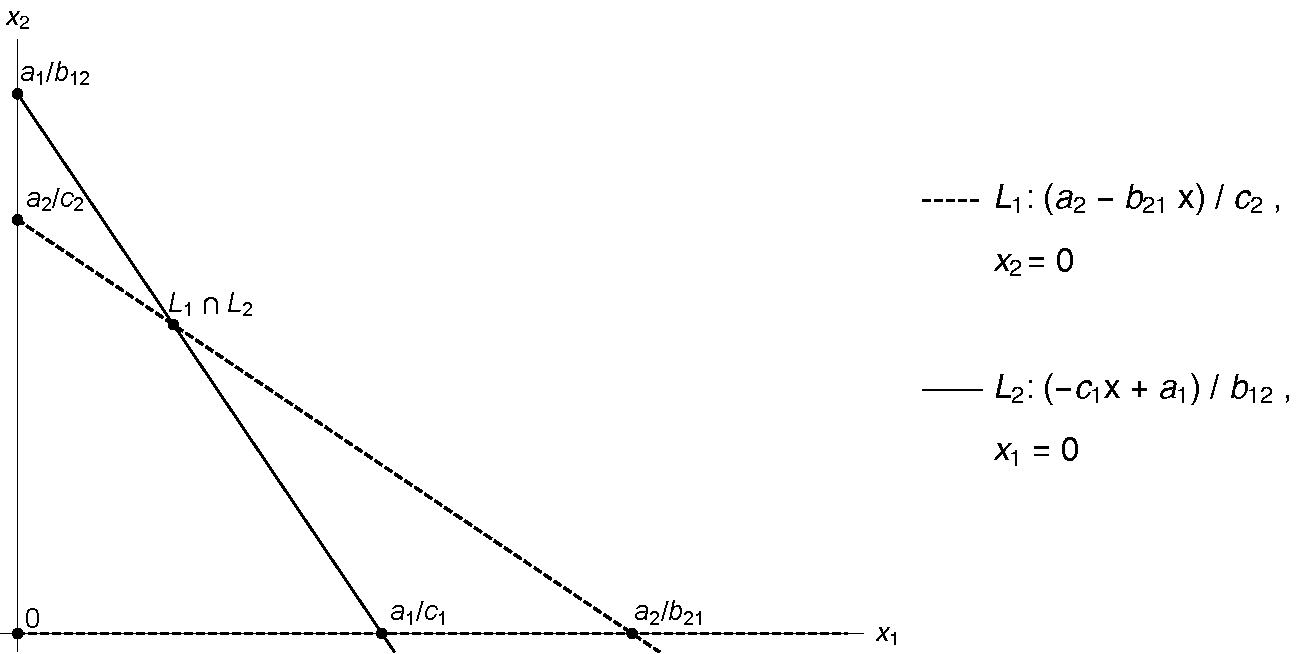
\includegraphics[width=0.6\textwidth]{sep_1.pdf}
            \caption{Расположение прямых при указанных коэффициентах}
        \end{figure}
    \end{frame}

    \begin{frame}
        \begin{enumerate}
            \setlength\itemsep{0.5em}
            \item $ \lambda_1 = a_1 > 0,\ \lambda_2 = a_2 > 0 \Rightarrow $ точка $ {\rom 1} $ --- неустойчивый узел.     
            \item $ \lambda_1 = -a_1 < 0,\ \lambda_2 = \dfrac{a_2 c_1 - a_1 b_{21}}{c_1} < 0 \Rightarrow $ точка $ {\rom 2} $ --- устойчивый узел.
            \item  $ \lambda_1 = \dfrac{a_1 c_2 - b_{12} a_2}{c_2} < 0,\ \lambda_2 = -a_2 < 0 \Rightarrow $ точка $ {\rom 3} $ --- устойчивый узел. 
            \item $ \det \mathbb{J}_{\rom 4}\! < \!0 \Rightarrow $ собственные значения имеют разные знаки, а значит точка $ {\rom 4} $ --- седло.
        \end{enumerate}

        \begin{figure}
            \centering
            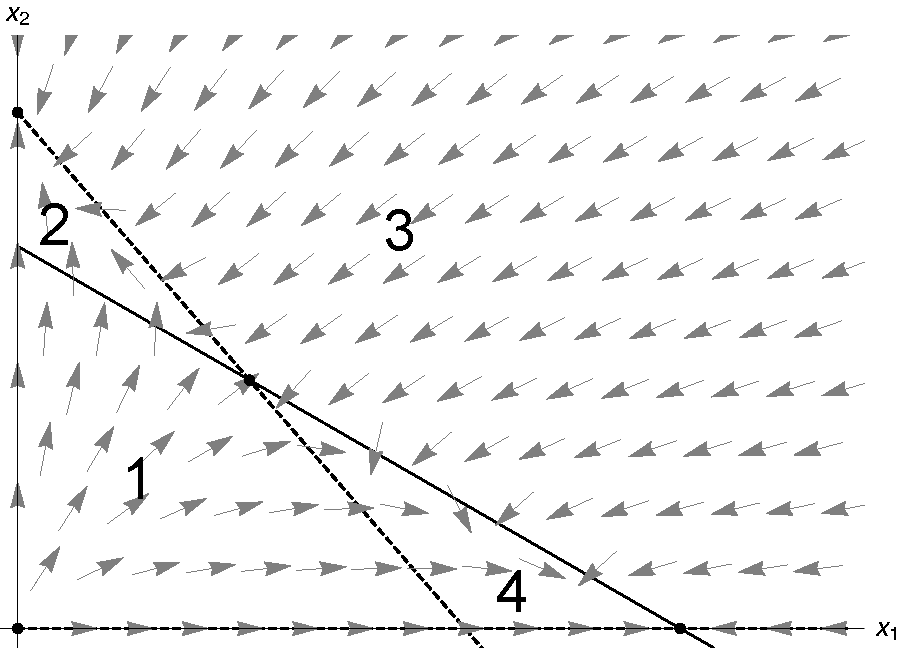
\includegraphics[width=0.45\textwidth]{areas_2.pdf}
            \caption{Поле направлений}
        \end{figure}
    \end{frame}

    \begin{frame}
        Значит, фазовый потрет выглядит следующим образом:
        \begin{figure}[h]
            \centering
            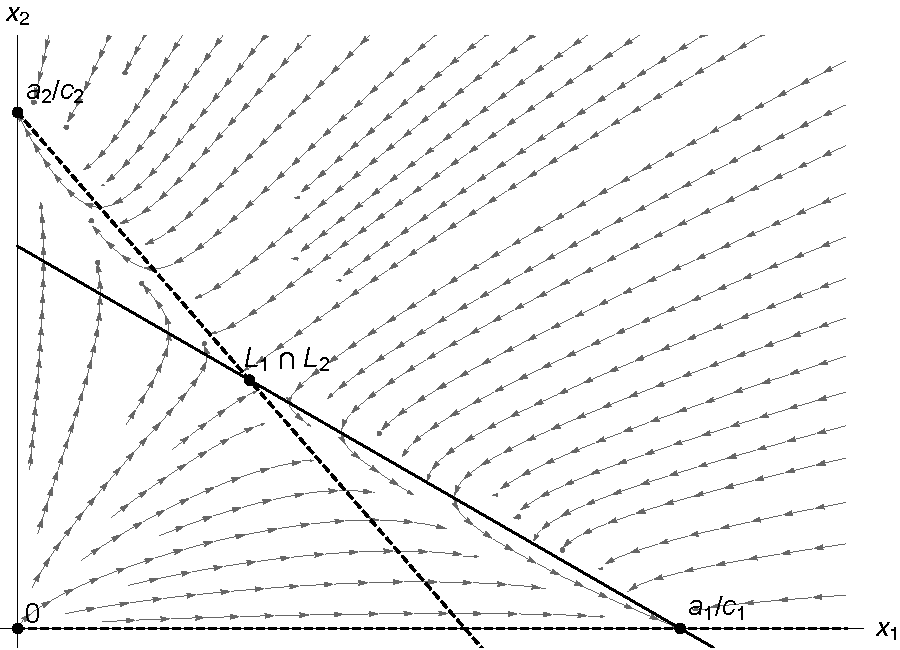
\includegraphics[width=0.6\textwidth]{phase_2.pdf}
            \caption{Выжывание одного из видов}
            \label{fig:phase_2}
        \end{figure}

        Большинство траекторий стремятся либо ко 2-ой, либо к 3-ей точке. А они соответствуют выживанию лишь одного из видов. Сосуществование крайне маловероятно.
    \end{frame}

    \begin{frame}
        \frametitle{Заключение}
        Имея экспериментально выведенные коэфициенты размножения, а также коэфициенты межвидовой и внутривидовой конкуренции, мы можем построить модель взаимодействия между особями двух видов и понять, способны ли они сосуществовать или же один из них вымрет. Анализ особых точек (иными словами --- стационарных состояний) дает нам возможность построить график траекторий, чтобы определить, к какому из четырех стационарных состояний стремится система.
    \end{frame}

    \begin{frame}
        \frametitle{Список использованных источников}
        \begin{thebibliography}{9}
            % \bibitem{Loyts} Лойцянский Л.\,Г. Механика жидкости и газа. М.: Дрофа, 2003. 846 с.

            \bibitem{Model} Ризниченко Г.\,Ю. Лекции по математическим моделям в биологии. --- 2-е изд. испр. и доп. --- М. --- Ижевск: Институт компьютерных исследований, НИЦ <<Регулярная и хаотическая динамика>>. 2010. 560 с.

            \bibitem{agafonov} Агафонов С.А., Герман А.Д., Муратова Т.В. Дифференциальные уравнения. М.: Изд-во МГТУ им. Н.Э. Баумана, 1997. 336 с.

            \bibitem{petrovsky} Петровский И.Г. Лекции по теории обыкновенных дифференциальных уравнений. М.: Наука. 1970. 280 с.

            \bibitem{pentryagin} Понтрягин Л.С. Обыкновенные дифференциальные уравнения. М.: Наука. 1970. 332 с.

            \bibitem{samarsky} Самарский А.А., Гулин А.В. Численные методы. М.: Наука: Физматлит, 1989. 416 с.

        \end{thebibliography}
    \end{frame}
    


\end{document}